\begin{figure*}[!h]
\begin{subfigure}{0.18\linewidth}
\centering
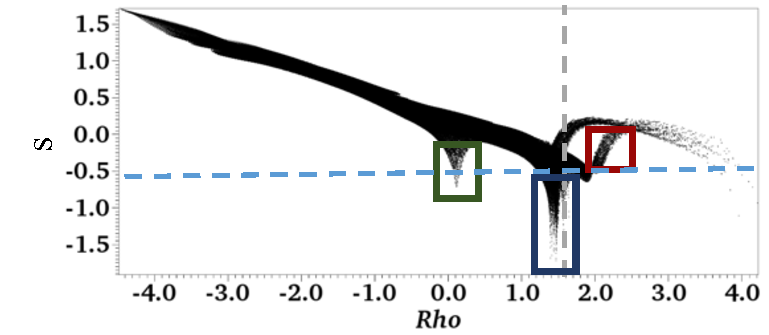
\includegraphics[width=\linewidth]{Images/EthaneDiol/scatterplot.pdf}
\caption{2D scatterplot of $\mathcal{A}$ and traits. We use $T = \left\{T_{A}, T_{B}, T_{C}, T_{D}\right\}$.} 
\vspace{-2mm}
\label{fig:ethanediol_scatterplot}
\end{subfigure}
\begin{subfigure}{0.16\linewidth}
\centering
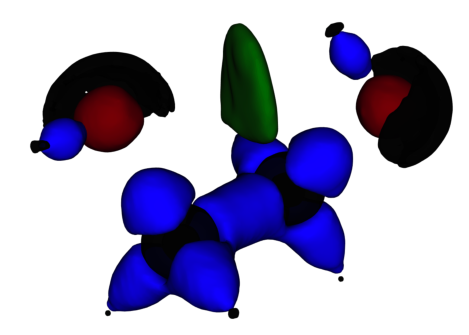
\includegraphics[width=\linewidth]{Images/EthaneDiol/zls.pdf}
\caption{$ZLS_{T}$}
\vspace{-2mm}
\label{fig:ethanediol_zls}
\end{subfigure}
\begin{subfigure}{0.16\linewidth}
\centering
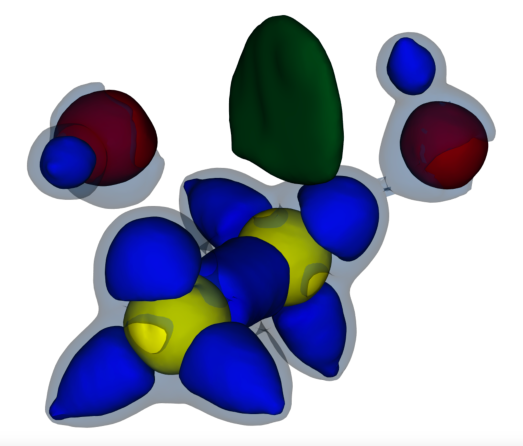
\includegraphics[width=\linewidth]{Images/EthaneDiol/fcls_cb_68.pdf}
\caption{+ $FCLS_{T_{A},68\%}$}
\vspace{-2mm}
\label{fig:ethanediol_fcls_cb}
\end{subfigure}
\begin{subfigure}{0.16\linewidth}
\centering
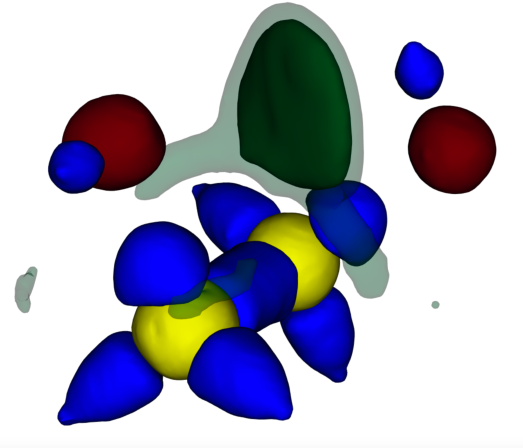
\includegraphics[width=\linewidth]{Images/EthaneDiol/fcls_ncb_68.pdf}
\caption{+ $FCLS_{T_{B},68\%}$}
\vspace{-2mm}
\label{fig:ethanediol_fcls_ncb}
\end{subfigure}
\begin{subfigure}{0.16\linewidth}
\centering
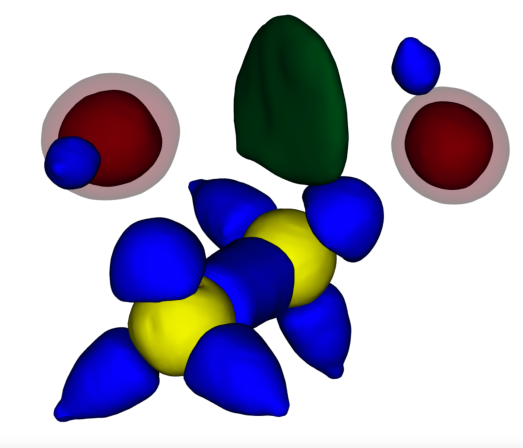
\includegraphics[width=\linewidth]{Images/EthaneDiol/fcls_oa_68.pdf}
\caption{+ $FCLS_{T_{C},68\%}$}
\vspace{-2mm}
\label{fig:ethanediol_fcls_oa}
\end{subfigure}
\begin{subfigure}{0.16\linewidth}
\centering
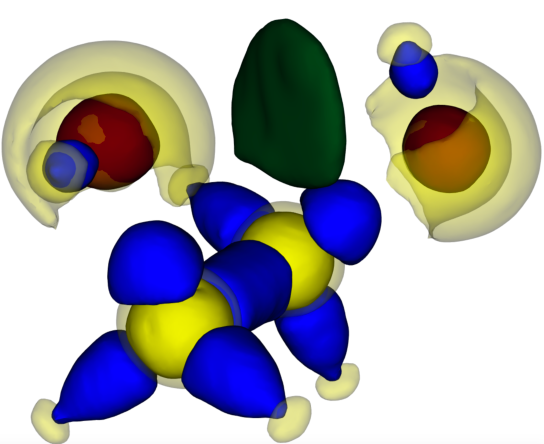
\includegraphics[width=\linewidth]{Images/EthaneDiol/fcls_ca_68.pdf}
\caption{+ $FCLS_{T_{D},68\%}$}
\vspace{-2mm}
\label{fig:ethanediol_fcls_ca}
\end{subfigure}
\caption{The covalent bonds~($T_{A}$, blue), non-covalent bond~($T_{B}$, green), oxygen atoms~($T_{C}$, red), and carbon atoms~($T_{D}$, yellow) of an ethanediol molecule are visualized using the electron density~(Rho) and reduced gradient~(s) attributes. These attributes are related exponentially in regions where no chemical interaction occurs and we selected our traits accordingly. In this case, we found $FCLS_{T,C}$ collectively visualized elements of the topological structure of the molecule.}
\vspace{-3mm}
\label{fig:ethanediol}
\end{figure*}
